\chapter{Protocol of work so far}
\section{Rotated lines experiment}

\subsection{Introduction}
The goal of this task was to recreate example 2 from \citet{nessler}. In this example they fed a winner-take-all spiking neural network images with lines in different orientations on them. The network then clustered the images into ten groups depending on their orientation.

\subsection{Methods}
\paragraph{Input data}
The images used in this task were generated with a size of 29 x 29 pixels. Black lines going through the center of the image were drawn onto a white background. To simulate noise each pixel had a chance of ten percent to have its color flipped. To ensure that all lines in the images have the same length regardless of their orientation a circular mask with a radius of 15 pixels was applied to the images. This recolored all pixels outside of the mask to white. During the training of the network these images were generated in uniformly distributed orientations for each training step and each image was shown for 200 ms. The random chosen orientation could lie between 0 and 359 degrees.  Two examples of such images can be seen in figure \ref{fig:angleImages}.

\begin{figure}
  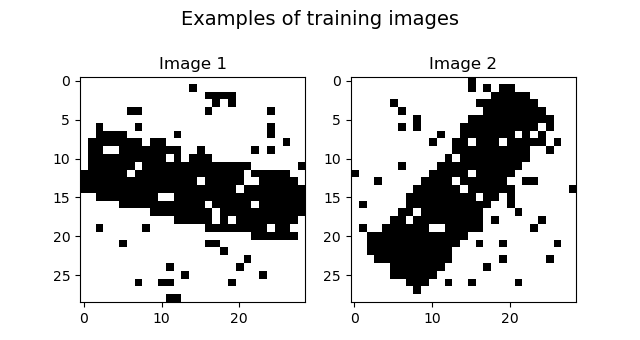
\includegraphics[width=\linewidth]{figures/angleNetwork/trainingImages.png}
  \caption{Two examples of the generated training data in this experiment.}
  \label{fig:angleImages}
\end{figure}

\paragraph{Neuron model}

As in \citet{nessler} the input neurons X are firing according to a poisson process with an average firing rate of 20 Hz when active and with 0 Hz when in an inactive state. The excitatory post synaptic potentials (EPSPs) $x_i(t)$ that these neurons produce can be seen in figure \ref{fig:XSpike}.

\begin{figure}
  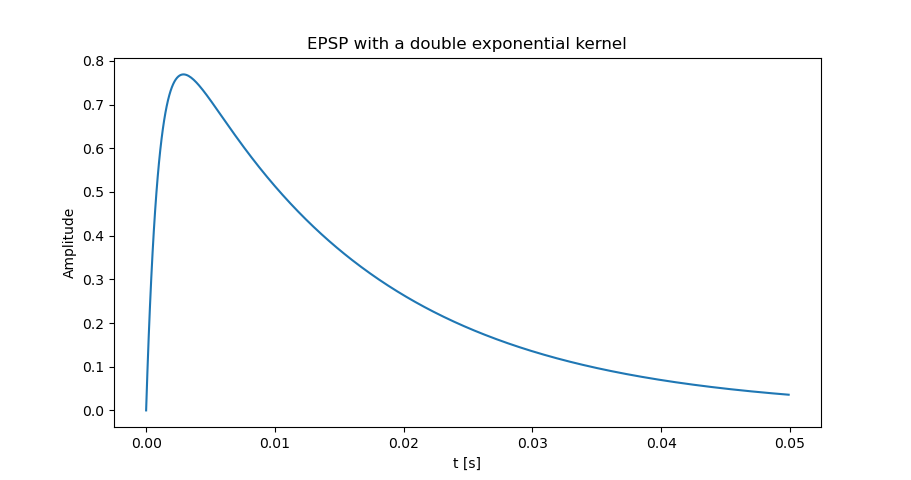
\includegraphics[width=\linewidth]{figures/XSpike.png}
  \caption{Form of an excitatory post synaptic potential generated by a X neuron over time. A double exponential kernel was used to generate this signal. These signals are fed to the next layer of the network. }
  \label{fig:XSpike}
\end{figure}

The firing rate of an output neuron $y_k$ depends exponentially on its membrane potential $U_k$ and the inhibitory signal $I_{inh}$ it receives. This can be seen in equation \ref{eqn:rk}. The chance of an individual Y neuron to fire within a time step $\delta t$ is given in equation \ref{eqn:rkdt}.

\begin{equation}
\label{eqn:rk}
r_k(t) = e^{u_k(t) - I(t)}
\end{equation}

\begin{equation}
\label{eqn:rkdt}
r_k(t) \cdot \delta t
\end{equation}

\paragraph{Network architecture}
Each pixel of an input image was connected to two neurons. The first of these neurons is in an active state when the pixel is black and in an inactive state otherwise. The second neuron expresses the opposite behaviour. As a consequence the network needs 1682 ($29 \cdot 29 \cdot 2$) excitatory input neurons $x_1,...,x_n$. These X neurons are fully connected to ten excitatory output neurons $y_1,...,y_k$. This means that that every input neuron $x_i$ is connected to each output neuron $y_k$. The membrane potential $U_k$ of each Y neuron is calculated by multiplying the EPSP of each X neuron times the weight of the connection between the X and Y neuron. 
\begin{equation}
\label{eqn:uk}
U_k(t) = \sum_{i=1}^n w_{ki} \cdot x_i(t)
\end{equation}
In \citet{nessler} each Y neuron also had an intrinsic excitability $w_{k0}$ which was learned for each neuron. For this experiment however it was omitted, as each orientation of input images was equally likely, thus the intrinsic excitability of each Y neuron would end up being the same.

The Y neurons are modelled in a winner-takes-all (WTA) circuit. This means that whenever one Y neuron spikes, a lateral inhibitory signal is fed to all Y neurons, thus preventing the further activation of all output neurons for $\sigma_{inh} = 5 ms$. After completion of the training of the network each Y neuron should be active for lines in an 18° area. 


\paragraph{Inhibition}
The inhibition signal was chosen to depend on the current membrane potential of the Y neurons. According to \citet{nessler} the overall firing rate of the Y neurons is:
\begin{equation}
\label{eqn:R}
R(t) = \sum_{k=1}^K e^{U_k(t) - I(t)}
\end{equation}
Solving this equation for I(t):
\begin{equation}
\label{}
R(t) = \frac{ \sum_{k=1}^K e^{U_k(t)}}{e^{I(t)}}
\end{equation}
\begin{equation}
\label{}
e^{I(t)} = \frac{\sum_{k=1}^K e^{U_k(t)}}{R(t)}
\end{equation}
\begin{equation}
\label{}
I(t) = \ln{ \frac{ \sum_{k=1}^K e^{U_k(t)}}{R(t)}}
\end{equation}
\begin{equation}
\label{eqn:I(t)}
I(t) =  - \ln{R(t)} + \ln{  \sum_{k=1}^K e^{U_k(t)}}
\end{equation}
When implementing the inhibition the $- \ln{R(t)}$ term of equation \ref{eqn:I(t)} was overlooked, that means it was assumed to be zero. Because of that R(t) equals 1 when the inhibition is active. This error was not detected at first, as the chance that a Y neuron fires within a time step of 1 ms with active inhibition is 1/1000 due to that oversight.

Whenever a Y neuron produces a spike the inhibition signal I(t) is subtracted from the membrane potential Uk(t) of every Y neuron. This happens for the duration of $\sigma_{inh} = 5 ms$. Thus follows:

\begin{equation}
\label{eqn:iinh}
I(t) = \begin{dcases*} \ln ( \sum_{i=1}^k e^{U_k} ) & if any $y_k$ fired in $ [t^f, t^f  + \sigma_{inh}] $ \\
0 & \text{if any $y_k$ did not fire in $ [t^f, t^f + \sigma_{inh}] $ } \end{dcases*}\end{equation}

\paragraph{Spike time dependent plasticity}
The weights $w_{ki}$ between neurons $x_i$ and $y_k$ are updated whenever a Y neuron fires. The time window $\sigma$ was set to 10 ms according to \citet{nessler}. If $y_k$ produces a spike all its weights are updated as follows:
\begin{equation}
\label{deltawki}
\Delta w_{ki} = \begin{dcases*} \lambda \cdot (ce^{-w_{ki}} - 1) & if $x_{i}$ fired in $ [t^f - \sigma, t^f] $ \\
\lambda \cdot (-1) & \text{if $ x_i $ did not fire in $ [t^f - \sigma, t^f] $ } \end{dcases*}
\end{equation}
\begin{tabbing}
\phantom{$c\ $}\= \kill
where:\> \\
$\lambda$\> ... learning rate \\
c\> ... shifts weights values \\
$t^f$\> ... time when $y_k$ spiked \\
$\sigma$ ... time window in which X spikes are considered as "before" Y spike
\end{tabbing}
As the membrane potentials U of the Y neurons result from the addition of the EPSPs of the 1682 X neurons times the corresponding weight, a way to control the average size of U is needed. If U is to small the output neurons will fire too sparsely and if U is too big it will impair the learning process. Thus to limit U the size of the weights is set via the parameter c. The learning rate $\lambda$ is needed to control the size of each weight update. If it is too big few Y neurons will take over more than the expected 18° areas and other Y will only respond for smaller areas or not at all. On the other hand if $\lambda$ is too small the network will learn very slowly and may never converge. Due to these two parameters being unwieldy to determine analytically they were chosen via grid search. 


\subsection{Results}

\paragraph{Parameter search}
The two parameters c, which controls the size of the weights, and the learning rate $\lambda$ were fitted to the network via grid search.	The tested parameters were as follows:
\begin{itemize}
  \item $c = 1$ ($\lambda = 10^{-2}, 10^{-3}, 10^{-4}$) 
  \item $c = 10$ ($\lambda = 10^{-2}, 10^{-3}, 10^{-4}$) 
  \item $c = 20$ ($\lambda = 10^{-2}, 10^{-2.5}, 10^{-3}, 10^{-3.5},  10^{-4}, 10^{-4.5}, 10^{-5}$) 
  \item $c = 30$ ($\lambda = 10^{-2}, 10^{-2.5}, 10^{-3}, 10^{-3.5}$) 
\end{itemize}
The simulation was conducted by simulating small discrete time steps and calculating the changes of the network in each step. The step size $\delta t$ was chosen as 1 ms.

\paragraph{$c = 1$}
The best results for $c = 1$ were achieved with $\lambda = 10^{-2}$. But overall this value for c did not work, even tough the network did learn to cluster images into eight groups depending on their orientation. In the image \ref{fig:c1Pie} you can see which Y neuron was the most active during the training process for each angle in 1° steps.

\begin{figure}
  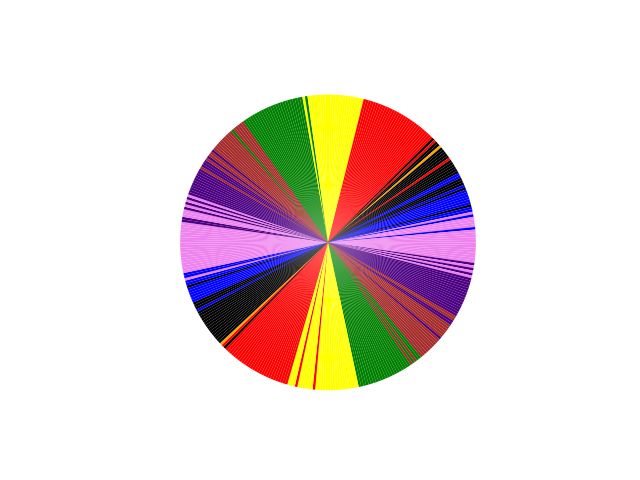
\includegraphics[width=\linewidth]{figures/angleNetwork/c1Pie.png}
  \caption{Most active Y neuron depending on orientation of the training image during the training process. $c = 1, \lambda = 10^{-2}$}
  \label{fig:c1Pie}
\end{figure}

However in figure \ref{fig:c1Distinct} the training progress of the network can be seen. The figure shows the number of distinct Y neurons active during the presentation of each training image shown. Due to the big, compared to other values of c, learning rate the network learned quickly. However after iteration 70 there were images shown for which not a single Y neuron spiked. This dying out of the networks activity is due to the parameter c being to small, which leads to too low membrane potentials.

\begin{figure}
  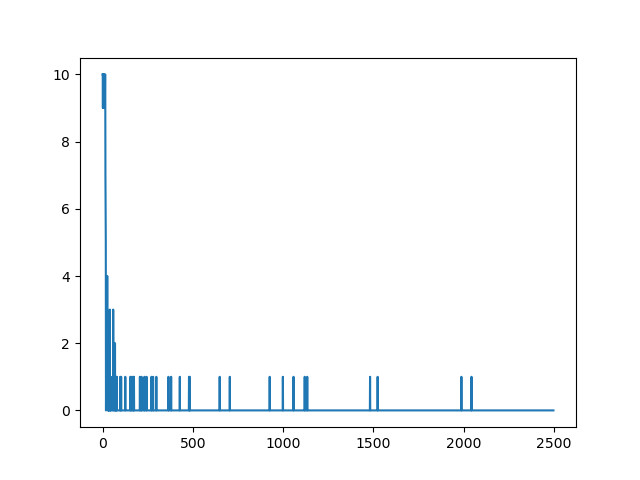
\includegraphics[width=\linewidth]{figures/angleNetwork/c1Distinct.png}
  \caption{Number of distinct Y neurons active during the presentation duration of each training image. x-axis: image shown, y-axis: distinct Y active, $c = 1, \lambda = 10^{-2}$}
  \label{fig:c1Distinct}
\end{figure}

\paragraph{$c = 10$}
This value of $c = 10$ had the same problem of the network activity dying out as $c = 1$ although at a later point in time, as can be seen in figure \ref{fig:c10Distinct}. Also in figure \ref{fig:c10LastSpikes} the last 50 Y spikes of the training process can be seen. As indicated by figure \ref{fig:c10Distinct} the activity is sparse.

\begin{figure}
  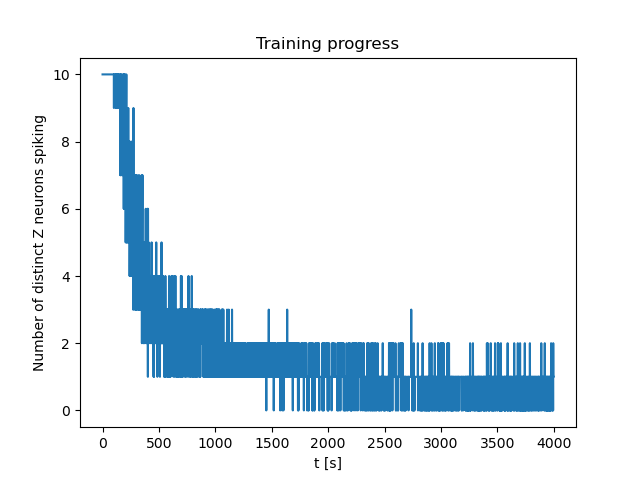
\includegraphics[width=\linewidth]{figures/angleNetwork/c10_3distinctZ.png}
  \caption{Number of distinct Y neurons active during the presentation duration of each training image. x-axis: image shown, y-axis: distinct Y active, $c = 10, \lambda = 10^{-3}$}
  \label{fig:c10Distinct}
\end{figure}

\begin{figure}
  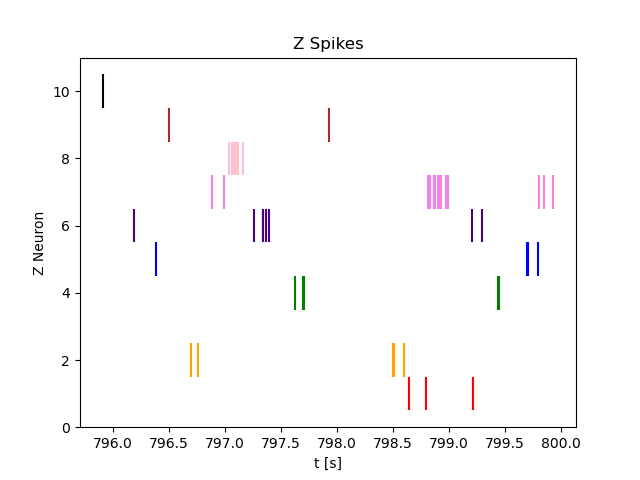
\includegraphics[width=\linewidth]{figures/angleNetwork/c10_3_50LastZSpikes.png}
  \caption{Last 50 Y neuron spikes, $c = 10, \lambda = 10^{-3}$}
  \label{fig:c10LastSpikes}
\end{figure}

\paragraph{$c = 20$}
$c = 20$ was the first value for which the network activity did not die out after some time. For $\lambda = 10^{-2}$ one Y neuron learned to spike first for every possible input image orientation, see figure \ref{fig:c20_2Pie}. 

\begin{figure}
  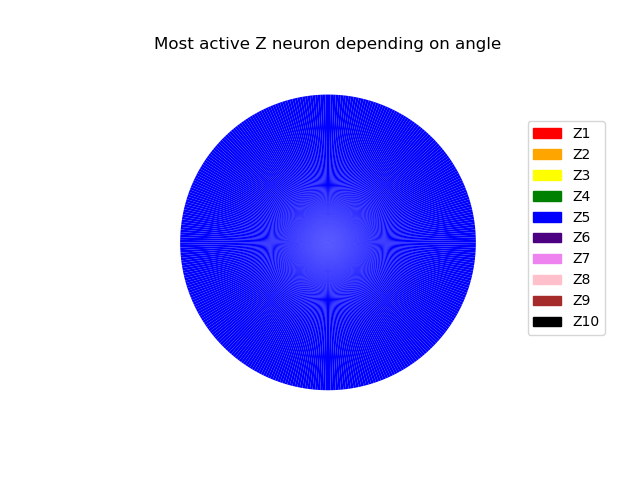
\includegraphics[width=\linewidth]{figures/angleNetwork/c20_2pie.png}
  \caption{Most active Y neuron depending on orientation of the training image during the training process. $c = 20, \lambda = 10^{-2}$}
  \label{fig:c20_2Pie}
\end{figure}

With $c = 20$ and $\lambda = 10^{-3}$ the first combination that yielded a stable network was found. In figure \ref{fig:c20_3Distinct} the amount of distinct Y neurons firing during the presentation of each training image can be seen. Figure \ref{fig:c20_3averageZ} shows the proportion of the most active Y neuron to all other Y neurons active for each training image. Both of these figures can be used to measure the training progress of the network. Figure \ref{fig:c20_3averageZ} however shows the additional information how certain the network is that a training image belongs to a specific group.

\begin{figure}
  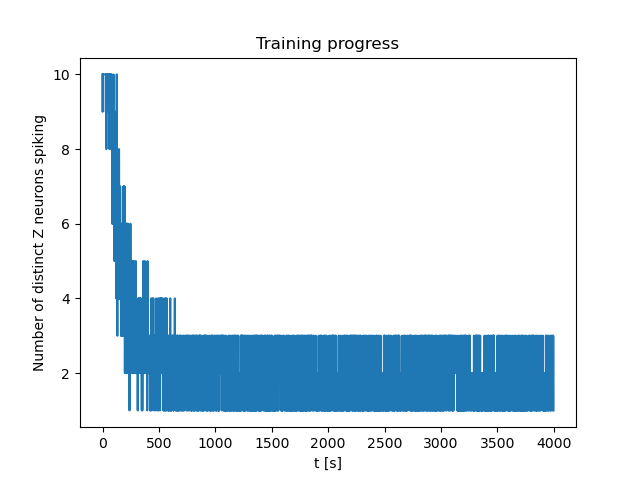
\includegraphics[width=\linewidth]{figures/angleNetwork/c20_3distinctZ.png}
  \caption{Number of distinct Y neurons active during the presentation duration of each training image. x-axis: image shown, y-axis: distinct Y active, $c = 20, \lambda = 10^{-3}$}
  \label{fig:c20_3Distinct}
\end{figure}

\begin{figure}
  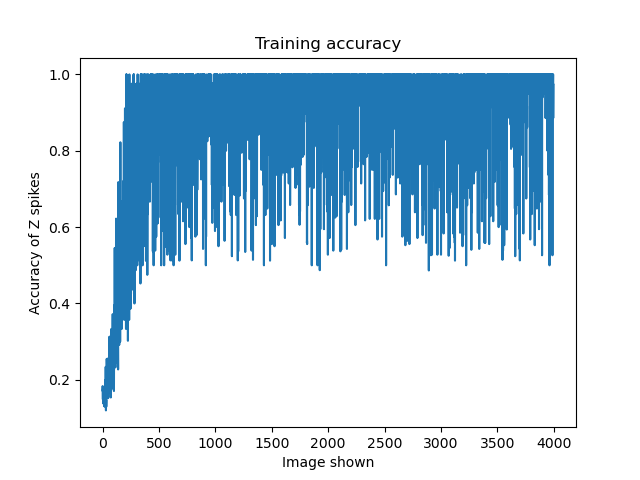
\includegraphics[width=\linewidth]{figures/angleNetwork/c20_3averageZ.png}
  \caption{Proportion (accuracy) of most active Y neuron  to activity of all other Y neurons during the presentation duration of each training image. $c = 20, \lambda = 10^{-3}$}
  \label{fig:c20_3averageZ}
\end{figure}

As this network did not die out after some time the trained network was analysed further. 180 images were generated in 1° steps and each was shown to the network for 200 ms. During each image presentation duration the most active Y neuron was recorded. This yielded figure \ref{fig:c20_3Pie}.

\begin{figure}
  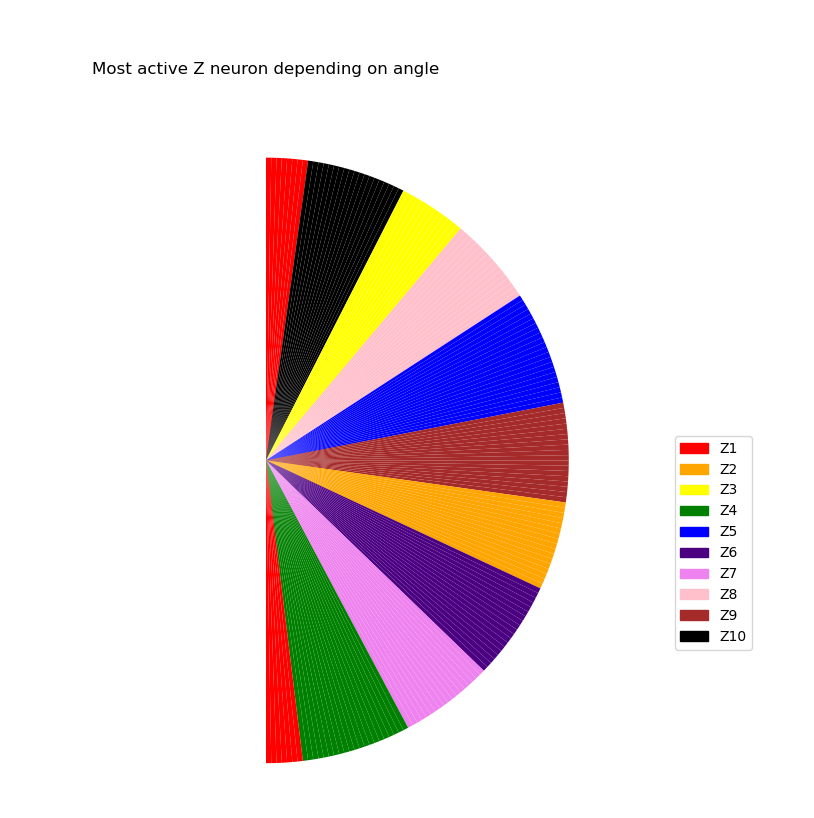
\includegraphics[width=\linewidth]{figures/angleNetwork/c20_3validationPie.png}
  \caption{Most active Y neuron depending on orientation of the training image during the training process. $c = 20, \lambda = 10^{-3}$}
  \label{fig:c20_3Pie}
\end{figure}

Also the number of distinct Y neurons firing during each image presentation was recorded and is shown in \ref{fig:c20_3validationDistinctZSpikes}. In this figure it is seems that the points in which there are three distinct Y neurons active are periodic in nature. This can be explained by figure \ref{fig:c20_3validationZSpikes}. There it can be seen that whenever the image orientation nears the border between two competing Y neurons both start to be active. This explains why for large parts of figure \ref{fig:c20_3validationDistinctZSpikes} 2 neurons are active. The the third distinct Y neuron the is occasionally active seems to be of stochastic nature as much of the lines in the images overlaps areas of many other Y neurons. However the occurrence of 3 distinct active Y neurons seems to mostly occur at or close to the border between two competing Y neurons, as there are already 2 distinct neurons firing by design.

\begin{figure}
  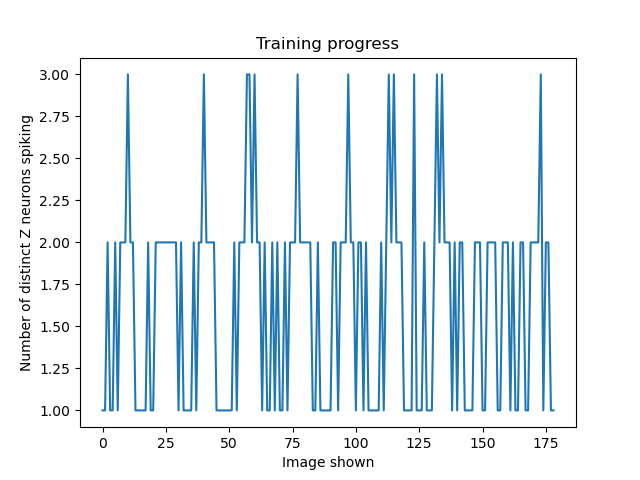
\includegraphics[width=\linewidth]{figures/angleNetwork/c20_3validationDistinctZSpikes.png}
  \caption{Number of distinct Y neurons active during the presentation duration of each training image. x-axis: image shown, y-axis: distinct Y active, $c = 20, \lambda = 10^{-3}$}
  \label{fig:c20_3validationDistinctZSpikes}
\end{figure}

valizspikes

\begin{figure}
  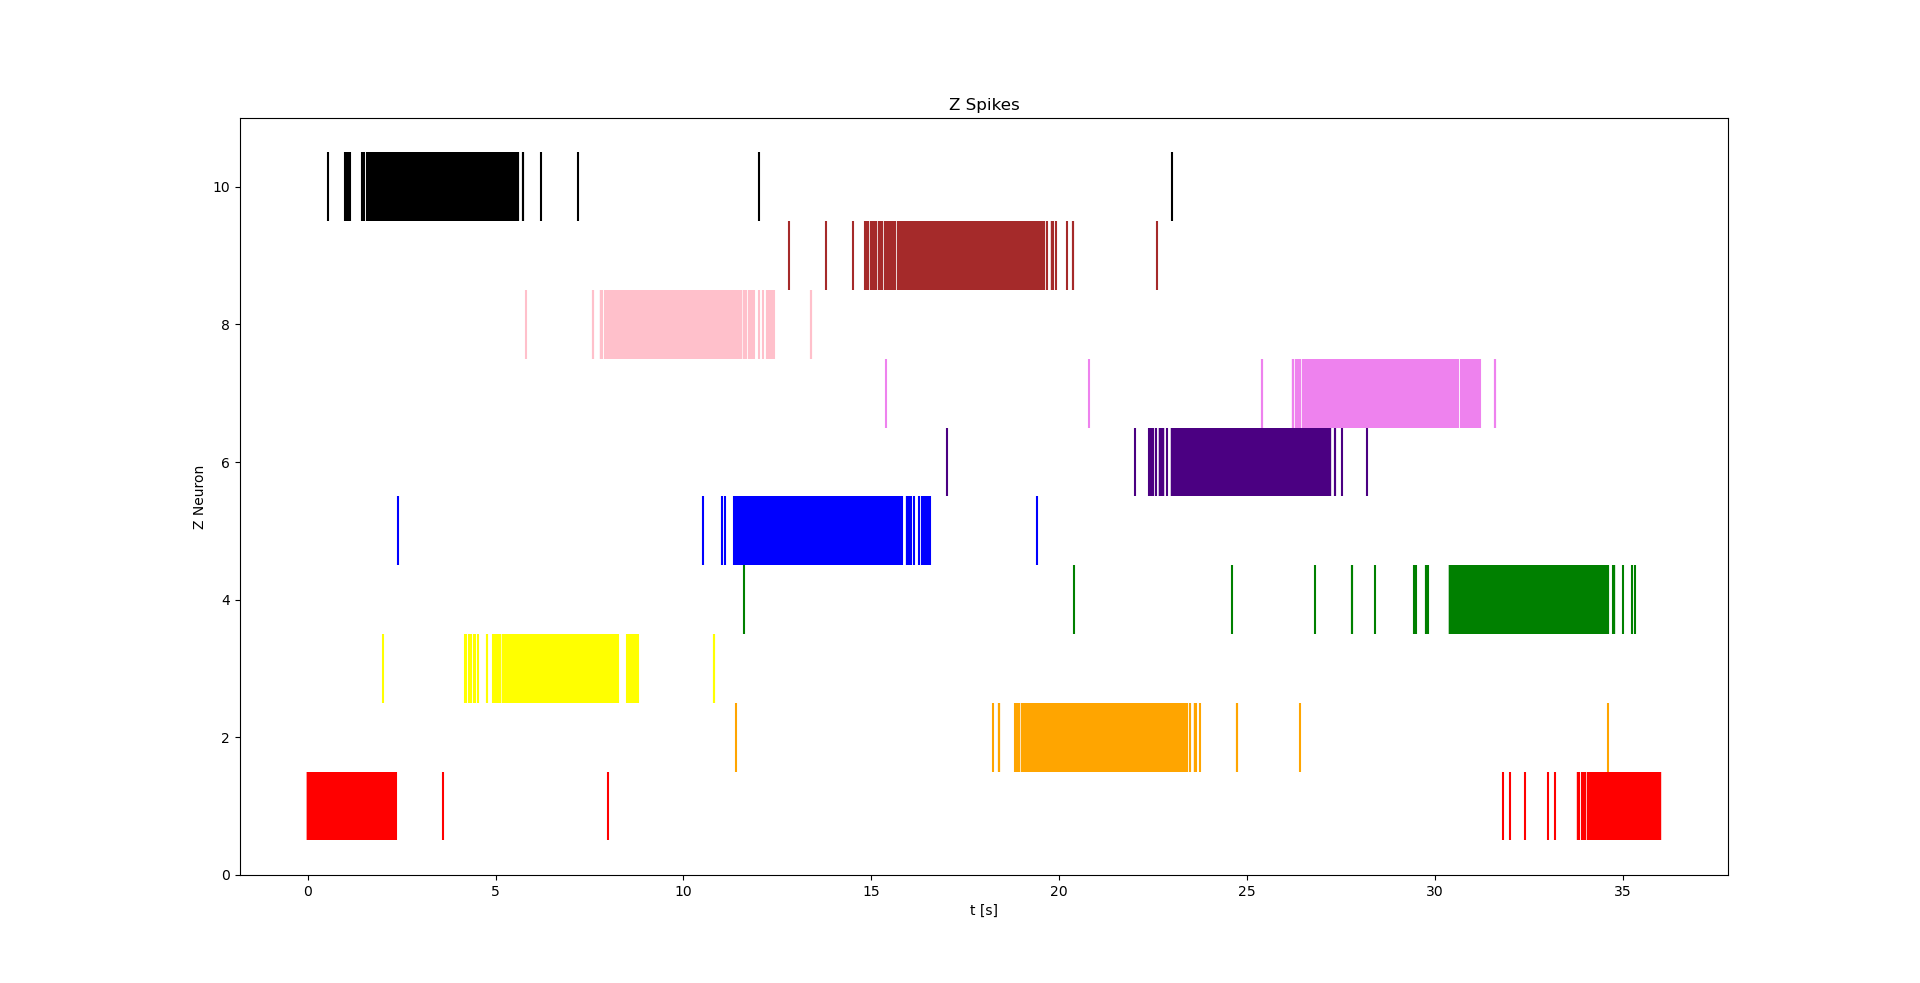
\includegraphics[width=\linewidth]{figures/angleNetwork/c20_3validationZSpikes.png}
  \caption{Y spikes over the presentation of input images from 0 to 179°, $c = 20, \lambda = 10^{-3}$}
  \label{fig:c20_3validationZSpikes}
\end{figure}

Also it was possible to project the learned weights $w_{ki}$ into the 2-D space to observe what they represent. This projection can be seen in figure \ref{fig:c20_3weights2.png} for the weights of $y_10$.

\begin{figure}
  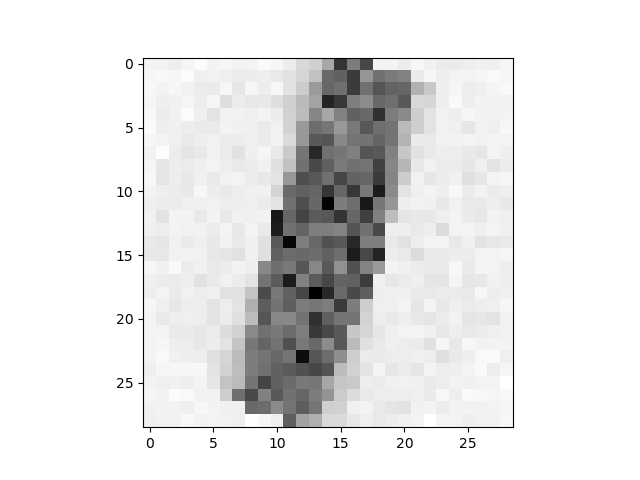
\includegraphics[width=\linewidth]{figures/angleNetwork/c20_3weights2.png}
  \caption{Visualization of the learned weights of $y_10$.}
  \label{fig:c20_3weights2.png}
\end{figure}

The results for smaller $lambda$ were also valid, but as they did not seem to be superior to the parameters $c = 20$ and $\lambda = 10^{-3}$. As with smaller learning rates the training simply took longer and the performance of the network did not improve they were discarded and  the learning rate $\lambda = 10^{-3}$ was declared winner for $c = 20$. To save space the figures of smaller learning rates will not be shown here.

\paragraph{$c = 30$}
$c = 30$ also yielded a functioning network, but it did perform analogous to $c = 20$. It did perform in the same way, as with $c = 20$ the Y neurons already fire every 5 ms, slowed down by the inhibition. By increasing c further the Y neuron did not increase their activity.

\subsection{Conclusion}

The parameters $c = 20$ and $\lambda = 10^{-3}$ were finally chosen as the network performed the best and trained the quickest with these parameters, without raising the membrane potential needlessly.

%\section{Horizontal and vertical lines experiment}
